%=========================================================
\chapter{Modelado Estático}	
\label{cap:reqSist}

	En este capítulo se modela la {\em Arquitectura del negocio} la cual está conformada por la Ontología del negocio ({\em Términos} y {\em Hechos del negocio}), Arquitectura de procesos y las {\em Reglas del negocio}. Primero se especifica brevemente el {\em Contexto} en el que los términos tienen significado.
	
	En las secciones \ref{sec:terminosDeNegocio} y \ref{sec:hechosDeNegocio} se presentan los Términos del negocio a manera de Glosario y por último se presentan los Hechos del negocio a manera de relaciones entre términos del negocio.

%----------------------------------------------------------
\section{Diseño de Subsistemas}

	\cdtInstrucciones{El contexto debe explicar bajo que ambiente los términos del negocio son aplicables y proporcionar información general para su comprensión inicial.\\}
	La empresa ``Fast Rent'' se dedica a la renta de vehículos automotores, principalmente automóviles y motocicletas. Los clientes rentan vehículos por tiempos determinados y la empresa se encarga de dar mantenimiento a los vehículos y administrarlos para que estén disponibles para sus clientes. Los empleados, se dedican a labores de gerencia, atención a clientes, mantenimiento y soporte para los vehículos activos.
	
%---------------------------------------------------------
\section{Diseño de Módulos}
\label{sec:terminosDeNegocio}
\begin{description}
	% Ejemplo de un término literal.
	\item[\hypertarget{tAutomovil}{Automóvil:}] ({\em es un tipo de \hyperlink{tVehiculo}{Vehículo}}) De cuatro ruedas con capacidad de 5 a 9 personas. 
	% Ejemplo de un término de entidad
	\item[\hypertarget{tCliente}{Cliente:}] Se refiere a todas las personas físicas y morales que \hyperlink{tRenta}{rentan} o han rentado un \hyperlink{tVehiculo}{vehículo}.
	
	\item[\hypertarget{tDirector}{Director:}] ({\em es un tipo de \hyperlink{tEmpleado}{Empleado}}) Es el empleado que tiene mayor rango de todos y no tiene superior, a diferencia de los demás.	
	\item[\hypertarget{tEmpleado}{Empleado:}] Se refiere a cualquier persona que labore en la empresa.
	
	\item[\hypertarget{tChecador}{Checador:}] ({\em Reloj asociado al atributo:} Hora de entrada y salida de un \hyperlink{tEmpleado}{empleado}. {\em Frecuencia de lectura:} Una vez al día para la entrada y otra para la salida durante los días laborales.
	
	\item[\hypertarget{tMotocicleta}{Motocicleta:}] ({\em es un tipo de {tVehiculo}{Vehículo}}) De dos ruedas con capacidad para una personas. 

	\item[\hypertarget{tRenta}{Renta:}] Se refiere al servicio que ofrece la empresa para prestar \hyperlink{tVehiculo}{vehículos} a los \hyperlink{tCliente}{clientes} por un tiempo definido.
	
	\item[\hypertarget{tVehiculo}{Vehiculo:}] Se refiere a los automóviles y motocicletas que la empresa usa para dar el servicio de renta a los \hyperlink{tCliente}{clientes}.
	
%	\brTermSensor{tVelocimetro}{Velocímetro:}{Velocidad de un Vehículo.}{Kilometros/hora.}{Constantemente siempre que el \cdtRef{tVehiculo}{vehículo} esté encendido.}
\end{description}

%----------------------------------------------------------
\section{Diseño de Clases}
\label{sec:hechosDeNegocio}

%- - - - - - - - - - - - - - - - - - - - - - - - - - - - - 
\subsection{Modelo del dominio del problema}

	El modelo del dominio del problema se muestra en la figura~\ref{fig:modeloDeDominio}, a continuación se describen cada una de las entidades y sus relaciones.
	
\begin{figure}[htbp!]
	\begin{center}
		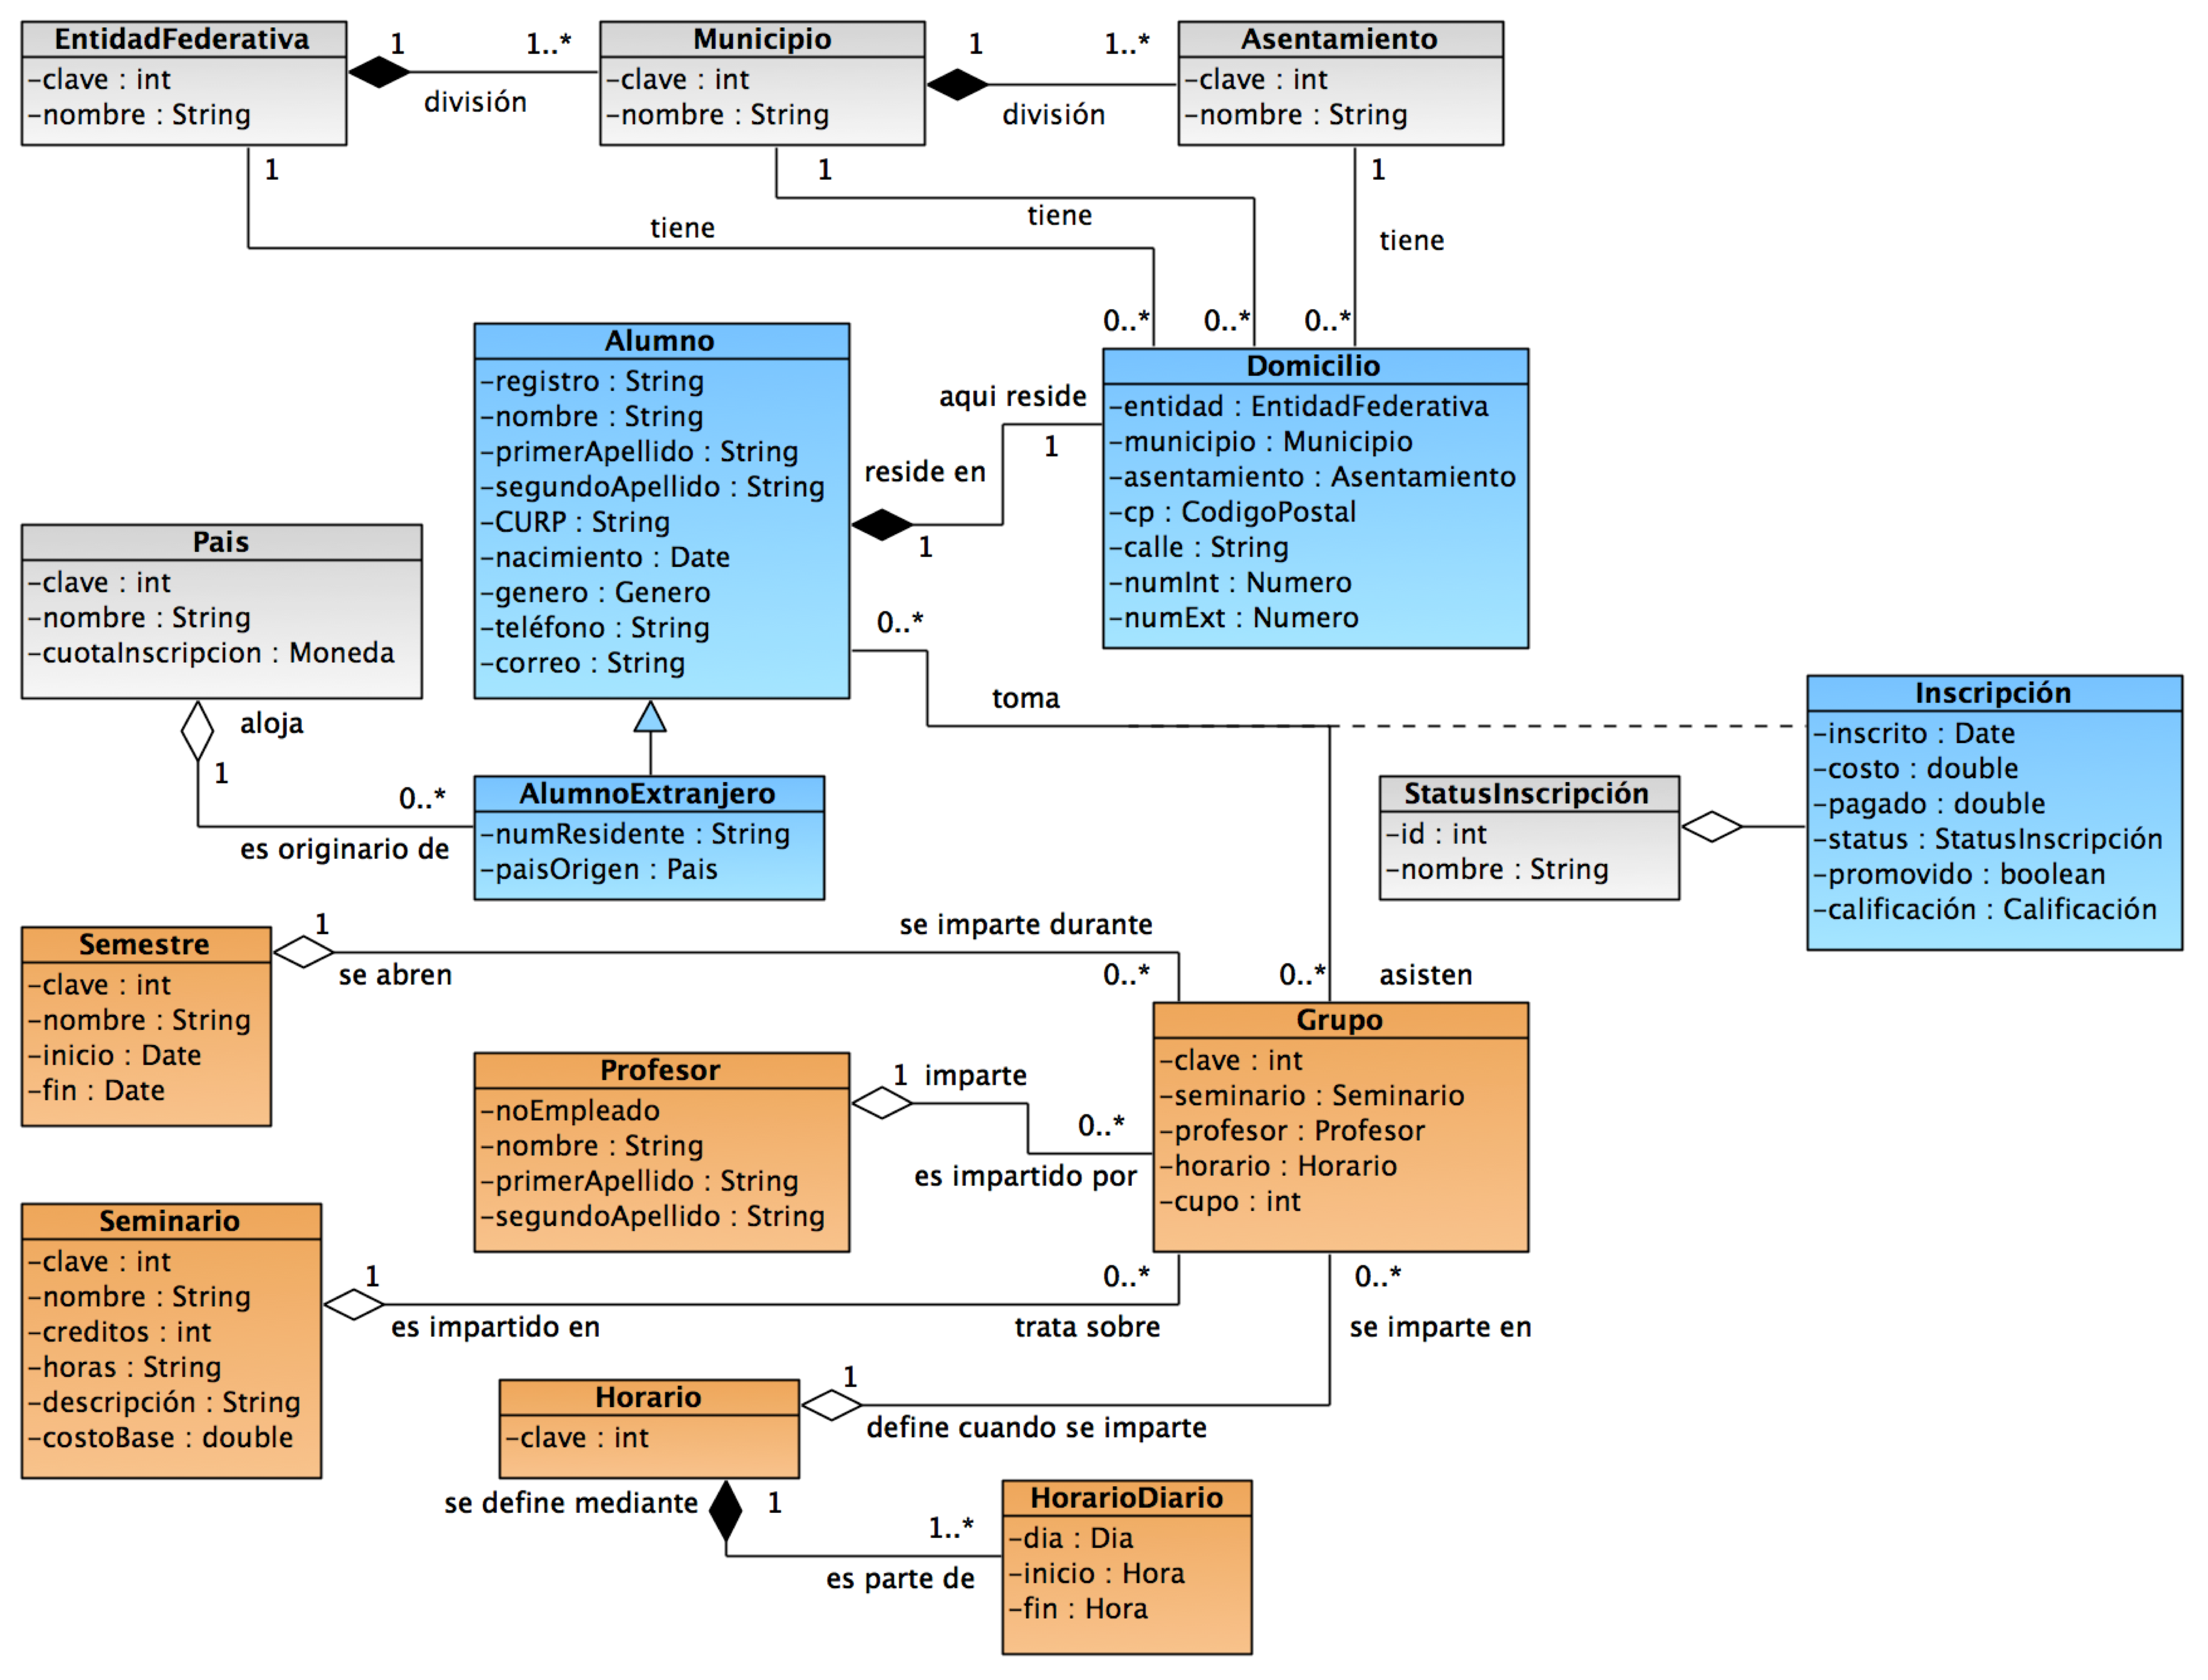
\includegraphics[angle=90,width=.95\textwidth]{images/modeloDelDominioDelProblema}
		\caption{Modelo del dominio del problema}
		\label{fig:modeloDeDominio}
	\end{center}
\end{figure}

%- - - - - - - - - - - - - - - - - - - - - - - - - - - - - 
\newenvironment{cdtEntidad}[2]{%
	\def \varBusinessEntityId{#2}%
	\hypertarget{#1}{\hspace{1pt}}%
	\newline%
	\noindent{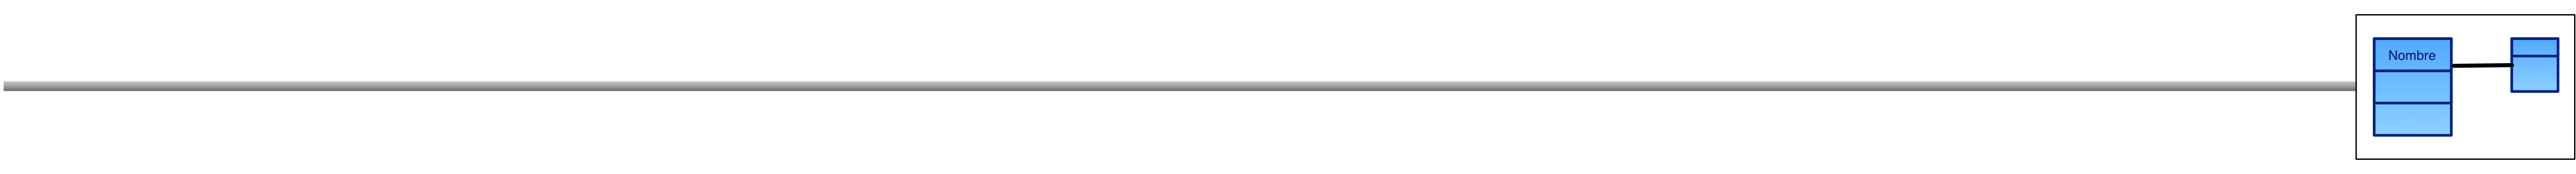
\includegraphics[width=\textwidth]{images/uc/classRule}}%
	\vspace{-25pt}%
	\subsection{Entidad: #2}%
	\noindent\begin{longtable}{|p{.2\textwidth}| p{.15\textwidth} | p{.46\textwidth} |p{.08\textwidth} |}%
	\hline%
	\multicolumn{4}{|c|}{{\cellcolor{colorSecundario}\color{white}Atributos}}\\ \hline%
	{\cellcolor{colorAgua}Nombre} &%
	{\cellcolor{colorAgua}Tipo} &%
	{\cellcolor{colorAgua}Descripción} &%
	{\cellcolor{colorAgua}Requerido}%
	\\ \hline%
	\endhead%
}{%
	\end{longtable}%
}

\newcommand{\brAttr}[5]{%
	{\bf\hypertarget{\varBusinessEntityId:#1}{#2}} & {\em{#3}} & {#4} & #5 \\\hline
}

\newcommand{\cdtEntityRelSection}{%
	\multicolumn{4}{|c|}{{\cellcolor{colorSecundario}\color{white}Relaciones}}\\ \hline%
	{\cellcolor{colorAgua}Tipo de relación} &%
	{\cellcolor{colorAgua}Entidad} &%
	\multicolumn{2}{|c|}{{\cellcolor{colorAgua}Rol}}
	\\ \hline%
}

\newcommand{\brRelComposition}{{\color{colorPrincipal}$\Diamondblack$\hspace{-1pt}---Composición}}
\newcommand{\brRelAgregation}{{\color{colorPrincipal}$\Diamond$\hspace{-1pt}---Agregación}}
\newcommand{\brRelGeneralization}{{\color{colorPrincipal}$\lhd$\hspace{-1pt}---Generalización}}

\newcommand{\brRel}[3]{%
	{\em{#1}} & {\bf{#2}} & \multicolumn{2}{|l|}{#3}\\\hline
}


%- - - - - - - - - - - - - - - - - - - - - - - - - - - - - 
\begin{cdtEntidad}{Alumno}{Alumno}
	\brAttr{registro}{Registro}{Id}{Número de registro utilizado para identificar un alumno}{Sí}
	\brAttr{nombre}{Nombre}{Palabra Corta}
		{Nombre o nombres del alumno.}{Sí}
	\brAttr{primerApellido}{Primer apellido}{Palabra Corta}
		{Primer apellido del alumno.}{Sí}
	\brAttr{segundoApellido}{Segundo apellido}{Palabra Corta}
		{Segundo apellido del alumno.}{No}
	\brAttr{CURP}{CURP}{CURP}
		{CURP del alumno.}{Sí}
	\brAttr{nacimiento}{Nacimiento}{Fecha}
		{Fecha de nacimiento del alumno.}{Sí}
	\brAttr{genero}{Género}{Domicilio}
		{Género del alumno.}{No}
	\brAttr{telefono}{Teléfono}{Telefono}
		{Teléfono para contactar al alumno.}{Sí}
	\brAttr{correo}{Correo}{Correo}
		{Correo del alumno para enviar información académica y escolar y para recuperación de clave de acceso.}{Sí}
	\cdtEntityRelSection
	\brRel{\brRelComposition}{Domicilio}{Un \hyperlink{Alumno}{Alumno} reside en un \hyperlink{Domicilio}{Domicilio}}	
	\brRel{\brRelAgregation}{Grupo}{Un \hyperlink{Alumno}{Alumno} toma un \hyperlink{Curso}{Curso}}	
\end{cdtEntidad}

%- - - - - - - - - - - - - - - - - - - - - - - - - - - - - 
\begin{cdtEntidad}{AlumnoExtranjero}{Alumno Extranjero}%{}
	\brAttr{numeroResidente}{Numero de residente}{Id}{Número de registro dado por la Secretaría de Relaciones Exteriores a los extranjeros.}{Si}
	\brAttr{paisOrigen}{Pais origen}{\hyperlink{Pais}{País}}
		{País de origen del alumno extranjero.}{Sí}
	\cdtEntityRelSection
	\brRel{\brRelAgregation}{País}{Un \hyperlink{Alumno}{Alumno} es originario de un \hyperlink{Pais}{Pais}}	
	\brRel{\brRelGeneralization}{Alumno}{Un \hyperlink{AlumnoExtranjero}{Alumno Extranjero} es un  \hyperlink{Alumno}{Alumno}}	
\end{cdtEntidad}

%---------------------------------------------------------
\section{Modelado de Reglas de negocio}

\begin{BussinesRule}{BR8}{Fecha de Nacimiento correcta.}
	\BRitem[Tipo:] Regla de integridad referencial o estructural. 
				% Otras opciones para tipo: 
				% - Regla de integridad referencial o estructural. 
				% - Regla de operación, (calcular o determinar un valor.).
				% - Regla de inferencia de un hecho.
	\BRitem[Clase:] Habilitadora. 
				% Otras opciones para clase: Habilitadora, Cronometrada, Ejecutive.
	\BRitem[Nivel:] Control. % Otras opciones para nivel: Control, Influencia.
	\BRitem[Descripción:]	Las Fechas de Nacimiento que se registran en el SINACEM para cualquier Persona debe ser mayores al día Primero de Enero del año 1900 y menor a la Fecha Actual.
	\BRitem[Motivación:] Evitar fraudes al PRONIM por el registro de personas que no han nacido al momento de su registro.
	\BRitem[Sentencia:] $\forall p \in Persona \Rightarrow 01-Enero-1900~<~p.fechaDeNacimiento~<~fechaActual$.
	\BRitem[Ejemplo positivo:] Para el día 12 de Octubre del 2013, cumplen la regla: 		
        \begin{itemize}
        	\item 11 de Octubre del 2013
			\item 20 de Diciembre del 2010
			\item 2 de Enero del 1900
        \end{itemize}
	
	\BRitem[Ejemplo negativo:] Para el día 12 de Octubre del 2013, no cumplen la 
		\begin{itemize}
        	\item 12 de Octubre del 2013
			\item 20 de Diciembre del 2014
			\item 1 de Enero del 1900
			\item 31 de Diciembre del 1899
        \end{itemize}
	
	\BRitem[Referenciado por:] \hyperlink{CUCE3.2}{CUCE3.2}, \hyperlink{CUCE3.3}{CUCE3.3}.
\end{BussinesRule}

\begin{BussinesRule}{BR129}{Determinar si un Estudiante puede inscribir Seminario.} 
	\BRitem[Tipo:] Regla de integridad referencial o estructural. 
				% Otras opciones para tipo: 
				% - Regla de integridad referencial o estructural. 
				% - Regla de operación, (calcular o determinar un valor.).
				% - Regla de inferencia de un hecho.
	\BRitem[Clase:] Habilitadora. 
				% Otras opciones para clase: Habilitadora, Cronometrada, Ejecutive.
	\BRitem[Nivel:] Control. % Otras opciones para nivel: Control, Influencia.
	\BRitem[Descripción:] Un Estudiante requere del 80\% de créditos para inscribirse a un Seminario y no haber cursado y reprobado otro seminario.
	\BRitem[Ejemplo positivo:] 
	
	\BRitem[Ejemplo negativo:] 
	
	\BRitem[Referenciado por:] 
\end{BussinesRule}

\begin{BussinesRule}{BR130}{Determinar si un Estudiante puede inscribirse en un Seminario}
	\BRitem[Tipo:] Regla de inferencia de un hecho.
				% Otras opciones para tipo: 
				% - Regla de integridad referencial o estructural. 
				% - Regla de operación, (calcular o determinar un valor.).
				% - Regla de inferencia de un hecho.
	\BRitem[Clase:] Habilitadora. 
				% Otras opciones para clase: Habilitadora, Cronometrada, Ejecutive.
	\BRitem[Nivel:] Control. % Otras opciones para nivel: Control, Influencia.
	\BRitem[Descripción:] El Estudiante debe pertenecer a la Carrera del Seminario y debe haber Cupo en el grupo del Seminario.
	\BRitem[Ejemplo positivo:] 
	
	\BRitem[Ejemplo negativo:] 
	
	\BRitem[Referenciado por:] 
\end{BussinesRule}

\begin{BussinesRule}{BR143}{Validar el horario del estudiante}
	\BRitem[Tipo:] Regla de operación, (calcular o determinar un valor.).
				% Otras opciones para tipo: 
				% - Regla de integridad referencial o estructural. 
				% - Regla de operación, (calcular o determinar un valor.).
				% - Regla de inferencia de un hecho.
	\BRitem[Clase:] Habilitadora. 
				% Otras opciones para clase: Habilitadora, Cronometrada, Ejecutive.
	\BRitem[Nivel:] Control. % Otras opciones para nivel: Control, Influencia.
	\BRitem[Descripción:] Las Materias y Seminarios inscritos por el alumno, en un periodo específico, no pueden impartirse en el mismo día de la semana en horas traslapadas.
	\BRitem[Ejemplo positivo:] 
	
	\BRitem[Ejemplo negativo:] 
	
	\BRitem[Referenciado por:] 
\end{BussinesRule}

\begin{BussinesRule}{BR180}{Calcular costos del Estudiante}
	\BRitem[Tipo:] Regla de operación, (calcular o determinar un valor.).
				% Otras opciones para tipo: 
				% - Regla de integridad referencial o estructural. 
				% - Regla de operación, (calcular o determinar un valor.).
				% - Regla de inferencia de un hecho.
	\BRitem[Clase:] Habilitadora. 
				% Otras opciones para clase: Habilitadora, Cronometrada, Ejecutive.
	\BRitem[Nivel:] Control. % Otras opciones para nivel: Control, Influencia.
	\BRitem[Descripción:] Los servicios se cobran de la siguiente forma:
		\begin{Citemize}
			\item {\em Estudiantes Regulares:} Se les Cobran todos los servicios al 100\% de su costo.
			\item {\em Estudiantes becados:} Se les otorga un 80\% de descuento en el costo de todos los servicios (antes del IVA).
			\item {\em Estudiantes extranjeros:} Se les cobran los servicios al 200\% del costo registrado.
		\end{Citemize}
	\BRitem[Sentencia:] $\forall~e~\in~\mathbb{E}\textrm{studiantes}~\land~\forall~s~\in \mathbb{S}\textrm{eminario}~\Rightarrow$
		\begin{displaymath}
			Costo(e,s) = \left\{ \begin{array}{ll}
			s.costo & , si~e.tipo = \textrm{Estudiante regular}\\
			{s.costo}\over{5} & , si~e.tipo = \textrm{Estudiante becado}\\
			s.costo \cdot 2 & , si~e.tipo = \textrm{Estudiante extranjero}
			\end{array} \right.
		\end{displaymath}
	\BRitem[Ejemplo positivo:] 
	
	\BRitem[Ejemplo negativo:] 
	
	\BRitem[Referenciado por:] 
\end{BussinesRule}

\begin{BussinesRule}{BR45}{Calcular impuestos por seminario}
	\BRitem[Tipo:] Regla de operación, (calcular o determinar un valor.).
				% Otras opciones para tipo: 
				% - Regla de integridad referencial o estructural. 
				% - Regla de operación, (calcular o determinar un valor.).
				% - Regla de inferencia de un hecho.
	\BRitem[Clase:] Habilitadora. 
				% Otras opciones para clase: Habilitadora, Cronometrada, Ejecutive.
	\BRitem[Nivel:] Control. % Otras opciones para nivel: Control, Influencia.
	\BRitem[Descripción:] Los impuestos corresponden al 16\% correspondientes al IVA.
	\BRitem[Sentencia:] $Impuesto(e, s) = Costo(e, s)\cdot0.16$.
	\BRitem[Ejemplo positivo:] 
	
	\BRitem[Ejemplo negativo:] 
	
	\BRitem[Referenciado por:] 
\end{BussinesRule}

\begin{BussinesRule}{BR100}{Recibo del Estudiante por inscripción a Seminario.}
	\BRitem[Tipo:] Regla de operación, (calcular o determinar un valor.).
				% Otras opciones para tipo: 
				% - Regla de integridad referencial o estructural. 
				% - Regla de operación, (calcular o determinar un valor.).
				% - Regla de inferencia de un hecho.
	\BRitem[Clase:] Habilitadora. 
				% Otras opciones para clase: Habilitadora, Cronometrada, Ejecutive.
	\BRitem[Nivel:] Control. % Otras opciones para nivel: Control, Influencia.
	\BRitem[Descripción:] El  Recibo del Estudiante debe mostrar el total del costo con el siguiente desglose:
		\begin{displaymath}\begin{array}{lr}
			Costo: & \$ XXX.XX\\
			Descuento~aplicado~(YY\%): & \$ XXX.XX\\
			Subtotal: & \$ XXX.XX\\
			IVA~(16\%): & \$ XXX.XX\\\hline
			Total: & \$ XXX.XX
		\end{array}\end{displaymath}
	\BRitem[Sentencia:] $CostoTotal = Costo(e, s) + Impuesto(e, s)$.
	\BRitem[Ejemplo positivo:] 
	
	\BRitem[Ejemplo negativo:] 
	
	\BRitem[Referenciado por:] 
\end{BussinesRule}



%---------------------------------------------------------
\section{Modelo de Procesos AS-IS}

En esta sección se describen los procesos a mejorar con el sistema.

% - - - - - - - - - - - - - - - - - - - - - - - - - - - - 
\subsection{PROC-01 Análisis de requerimientos}

\begin{figure}[htbp]
	\begin{center}
		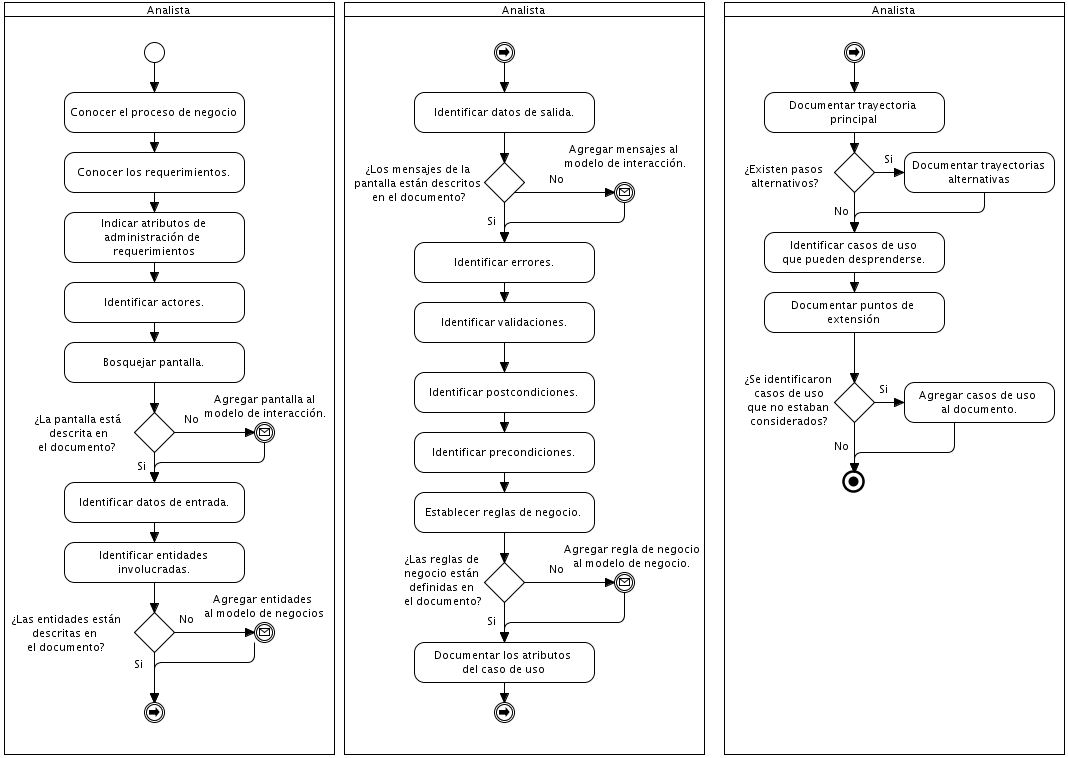
\includegraphics[width=.7\textwidth]{images/proceso1}
		\caption{PROC-01 Proceso de Análisis de requerimientos}
		\label{fig:proceso1}
	\end{center}
\end{figure}

\begin{description}
	\item[Descripción:] Describa el proceso indicando los aspectos relevantes que el diagrama no muestra.
	\item[Entradas:] \cdtEmpty
        \begin{itemize}
			\item Documentos de Procesos.
			\item Reglas de negocio.
			\item Minutas de las reuniones de análisis.
        \end{itemize}
	\item[Salidas:] \cdtEmpty
        \begin{itemize}
			\item Especificación de requerimientos.
			\item Bosquejo de pantallas.
			\item Modelo de base de datos
        \end{itemize}	
    \item[Áreas de oportunidad:] Liste los aspectos que detecta se pueden mejorar con la introducción del sistema o los problemas encontrados.
\end{description}

% - - - - - - - - - - - - - - - - - - - - - - - - - - - - 
\subsection{PROC-02 ...}

\begin{figure}[htbp]
	\begin{center}
		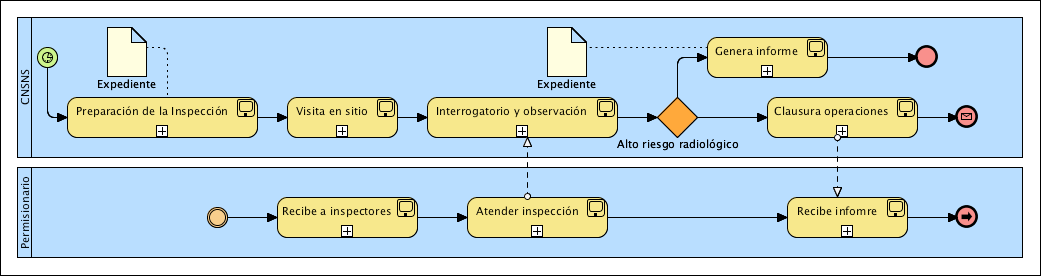
\includegraphics[width=.8\textwidth]{images/proceso2}
		\caption{PROC-02 Nombre del proceso}
		\label{fig:proceso2}
	\end{center}
\end{figure}

\begin{description}
	\item[Descripción:] ...
	\item[Entradas:] \cdtEmpty
        \begin{itemize}
			\item ...
        \end{itemize}
	\item[Salidas:] \cdtEmpty
        \begin{itemize}
			\item ...
        \end{itemize}	
    \item[Áreas de oportunidad:] Liste los aspectos que detecta se pueden mejorar con la introducción del sistema o los problemas encontrados.
\end{description}


%\input{proc/proc03.tex}
%\input{proc/proc04.tex}

%---------------------------------------------------------
\section{Modelo de procesos TO-BE}

Los nuevos procesos se presentan en esta sección, el mapa de procesos de se muestra en la figura~\ref{fig:mapaProc}.

\begin{figure}[htbp]
	\begin{center}
		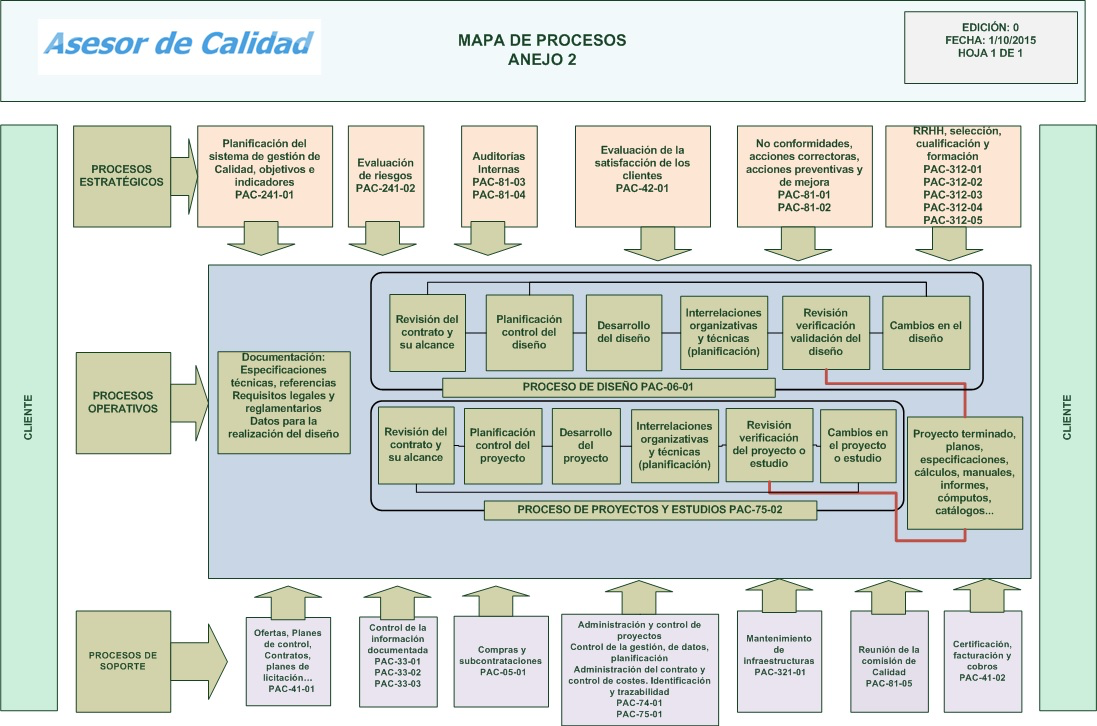
\includegraphics[width=.8\textwidth]{images/mapaProc}
		\caption{Mapa de procesos}
		\label{fig:mapaProc}
	\end{center}
\end{figure}


% - - - - - - - - - - - - - - - - - - - - - - - - - - - - 
\subsection{PROCM-01 ...}

\begin{figure}[htbp]
	\begin{center}
		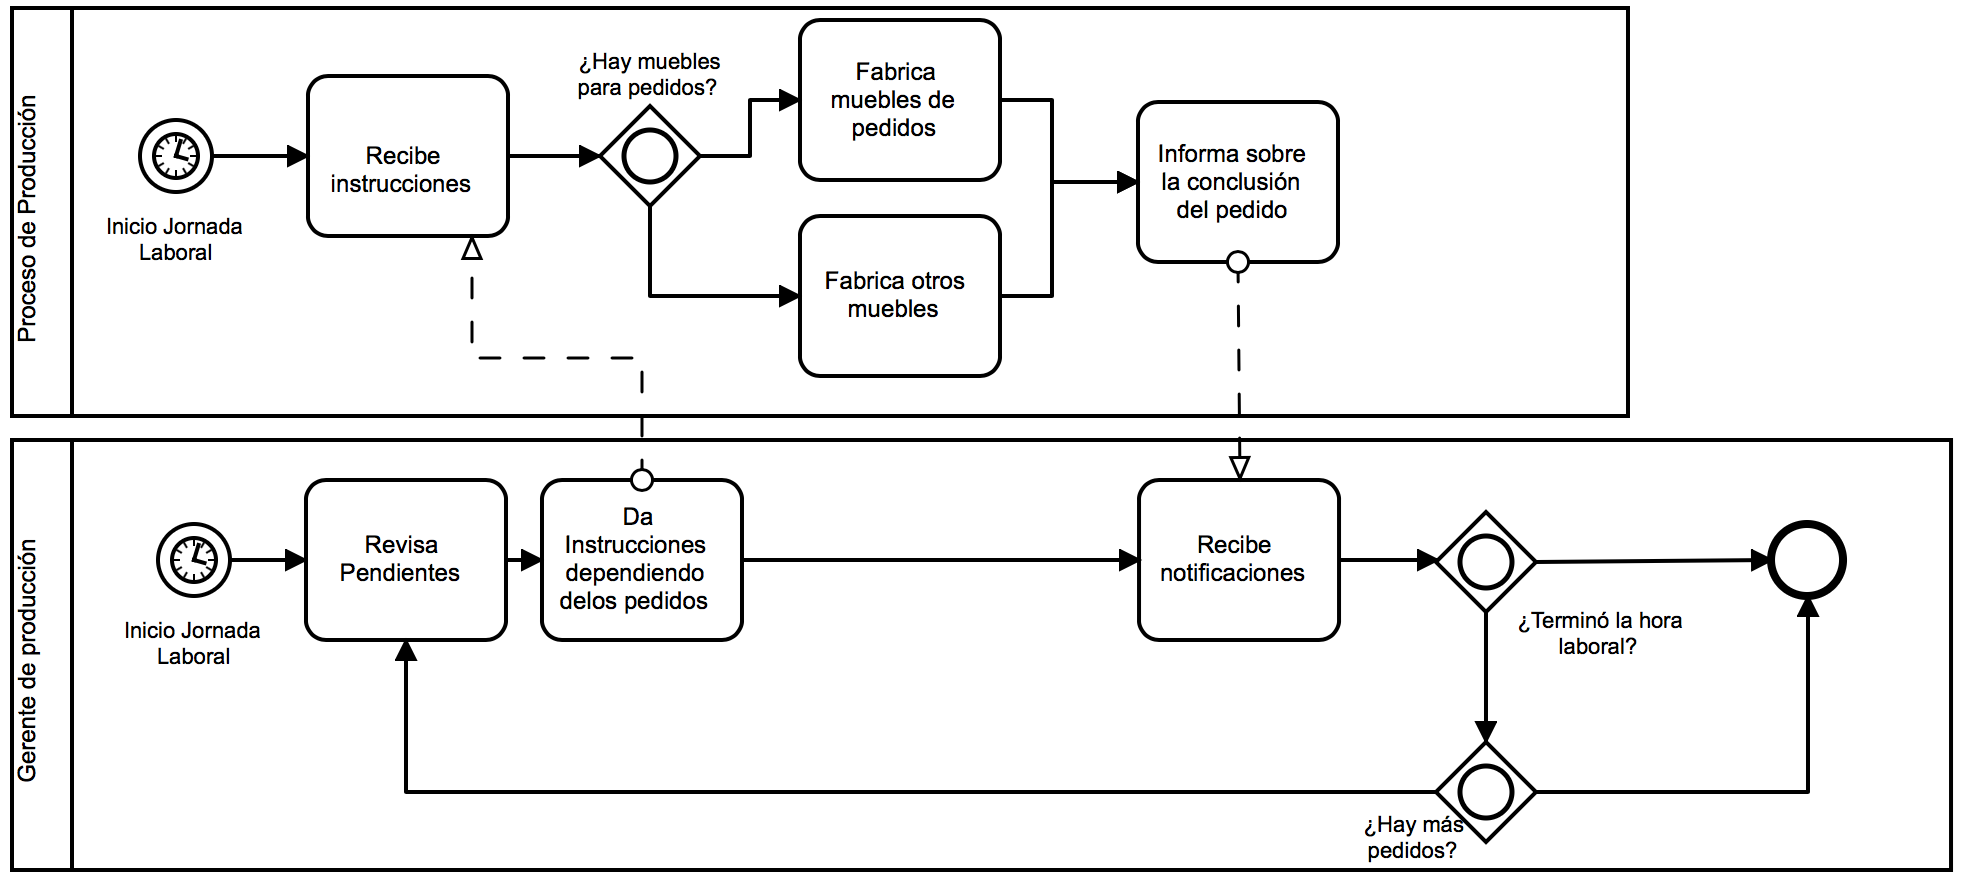
\includegraphics[width=.8\textwidth]{images/proceso3}
		\caption{PROCM-01 Nombre del proceso}
		\label{fig:proceso3}
	\end{center}
\end{figure}

\begin{description}
	\item[Descripción:] ...
	\item[Entradas:] \cdtEmpty
        \begin{itemize}
			\item ...
        \end{itemize}
	\item[Salidas:] \cdtEmpty
        \begin{itemize}
			\item ...
        \end{itemize}	
    \item[Mejoras esperadas:] Liste las mejoras que espera obtener tras la implementación del sistema.
    \item[Reglas de negocio:] \hyperlink{BR05}{BR05}, \hyperlink{BR8}{BR8}.
    \item[Casos de uso:] \hyperlink{CU3.4}{CU 3.4 Login}, \hyperlink{CU 4.3}{ CU 4.3 Consultar productos}.
\end{description}

%\input{proc/proc-m02.tex}
%\input{proc/proc-m03.tex}
%\input{proc/proc-m04.tex}

